% !TEX root = main.tex
%%%%%%%%%%%%%%%%%%%%%%%%%%%%%%%%%%%%%%%%%%%%%%%%%%%%%%
\section{実験方法および結果}
%%%%%%%%%%%%%%%%%%%%%%%%%%%%%%%%%%%%%%%%%%%%%%%%%%%%%%
実験装置を図の状態から90 [deg] 回転させ,初めに+方向に角速度を与えたときの角度推移を観測する.
実験を複数回行い,その平均値の角度推移をグラフにプロットする.また,同時に角速度の推移もプロットし,観測する.
\subsection{Duty比100\%・Duty比50\%による制御}
\subsubsection{実験方法}
 PWM信号のDuty比を,50\%と100\%にして実験を行う.


\subsubsection{実験結果}
 Duty比を50\%としたときの結果を図\ref{fig:fif}に,100\%としたときの結果を図\ref{fig:hund}に示す.
図に示すようにオーバーシュートが大きく,振動回数が2回となっている.
また,磁気トルカの発熱がひどく,磁気トルカの持つ抵抗による損失が大きいと考えられる.

\begin{figure}[h]
	\centering
	\begin{minipage}{0.43\columnwidth}
	  \centering
	  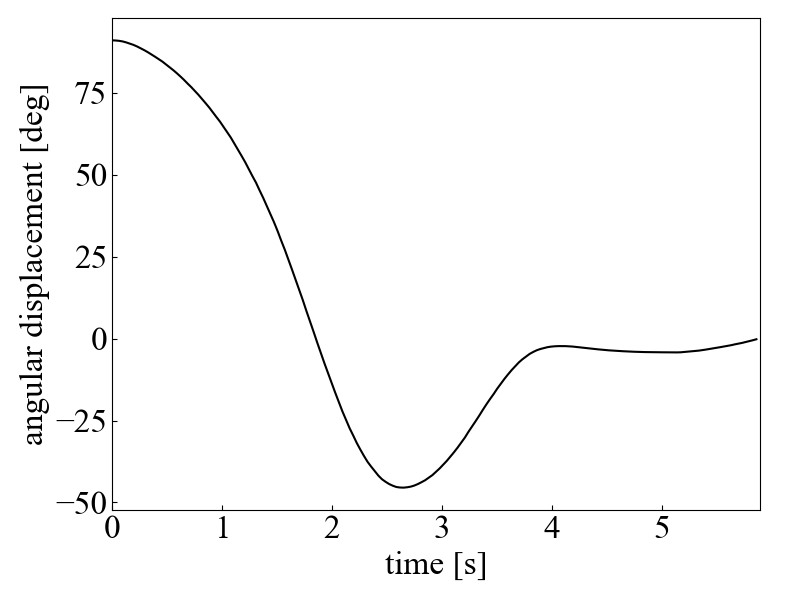
\includegraphics[width=\columnwidth]{./figure/duty50deg.png}
	  \caption{50\%としたときの角度推移}
	  \label{fig:duty50deg}
	\end{minipage}
	\hspace{5mm}
	\begin{minipage}{0.43\columnwidth}
	  \centering
	  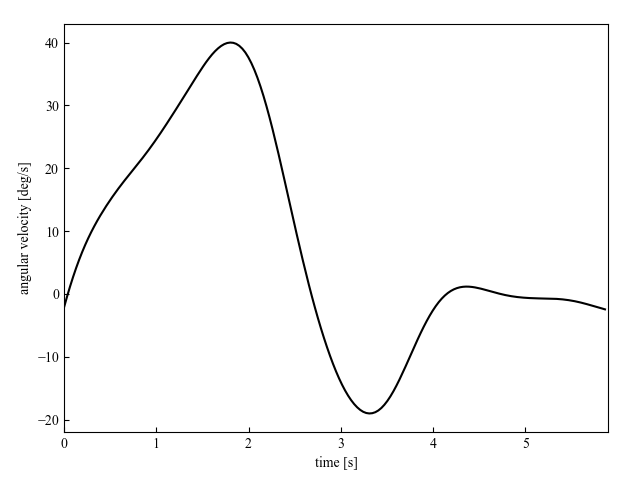
\includegraphics[width=\columnwidth]{./figure/duty50degpers.png}
	  \caption{50\%としたときの角速度推移}
	  \label{fig:duty50degpers}
	\end{minipage}
  \end{figure}

  \begin{figure}[h]
	\centering
	\begin{minipage}{0.43\columnwidth}
	  \centering
	  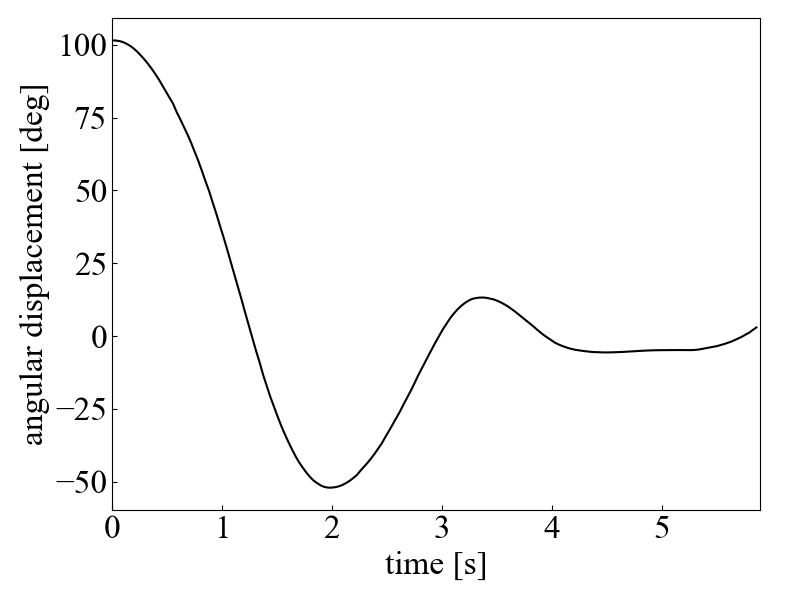
\includegraphics[width=\columnwidth]{./figure/duty100deg.png}
	  \caption{100\%としたときの角度推移}
	  \label{fig:duty100deg}
	\end{minipage}
	\hspace{5mm}
	\begin{minipage}{0.43\columnwidth}
	  \centering
	  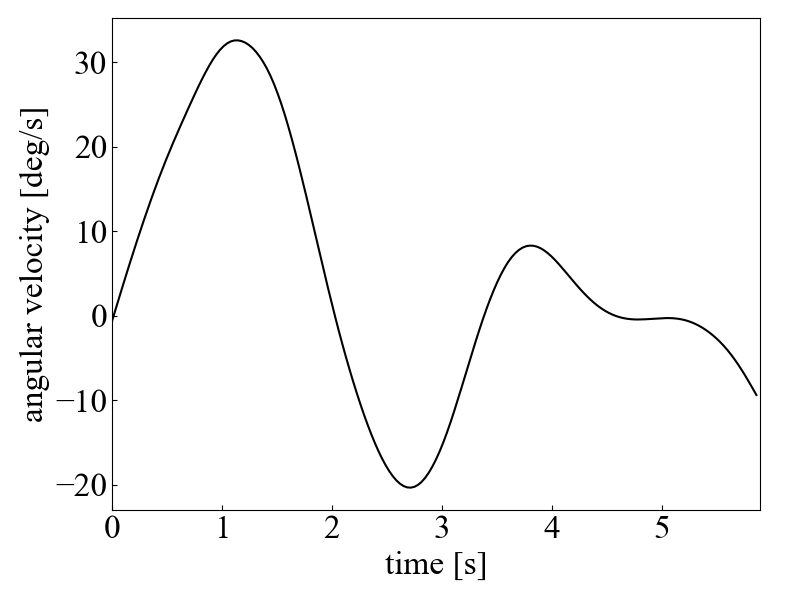
\includegraphics[width=\columnwidth]{./figure/duty100degpers.png}
	  \caption{100\%としたときの角速度推移}
	  \label{fig:duty100degpers}
	\end{minipage}
  \end{figure}

\newpage

\subsection{P制御}
\subsubsection{実験方法}
\subsubsection{実験結果}

\begin{figure}[h]
	\centering
	\begin{minipage}{0.43\columnwidth}
	  \centering
	  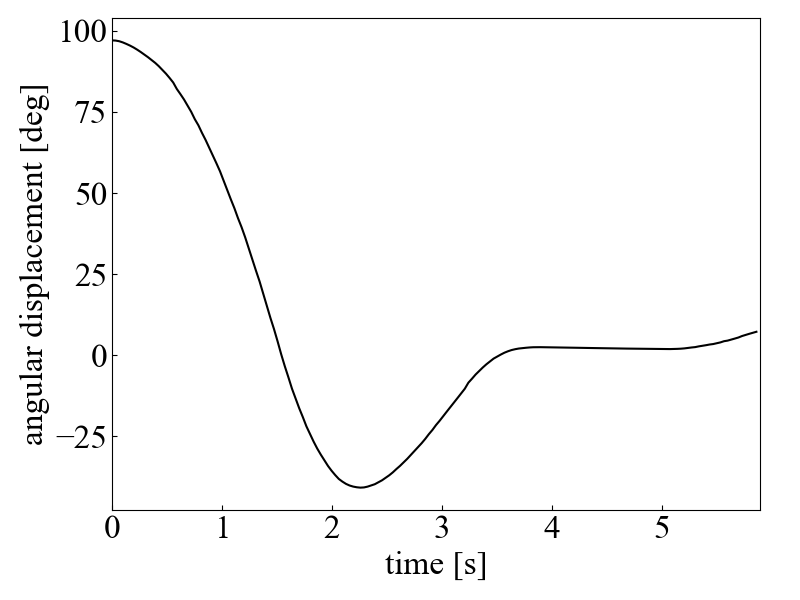
\includegraphics[width=\columnwidth]{./figure/Pdeg.png}
	  \caption{P制御の角度推移}
	  \label{fig:Pdeg}
	\end{minipage}
	\hspace{5mm}
	\begin{minipage}{0.43\columnwidth}
	  \centering
	  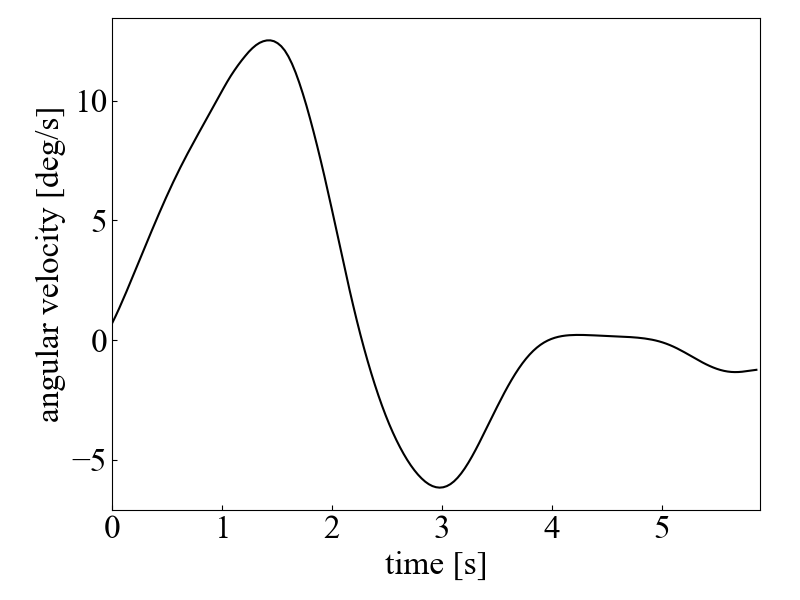
\includegraphics[width=\columnwidth]{./figure/Pdegpers.png}
	  \caption{P制御の角速度推移}
	  \label{fig:Pdegpers}
	\end{minipage}
  \end{figure}

\newpage

\subsection{P-D制御}
\subsubsection{実験方法}
\subsubsection{実験結果}

\begin{figure}[h]
	\centering
	\begin{minipage}{0.43\columnwidth}
	  \centering
	  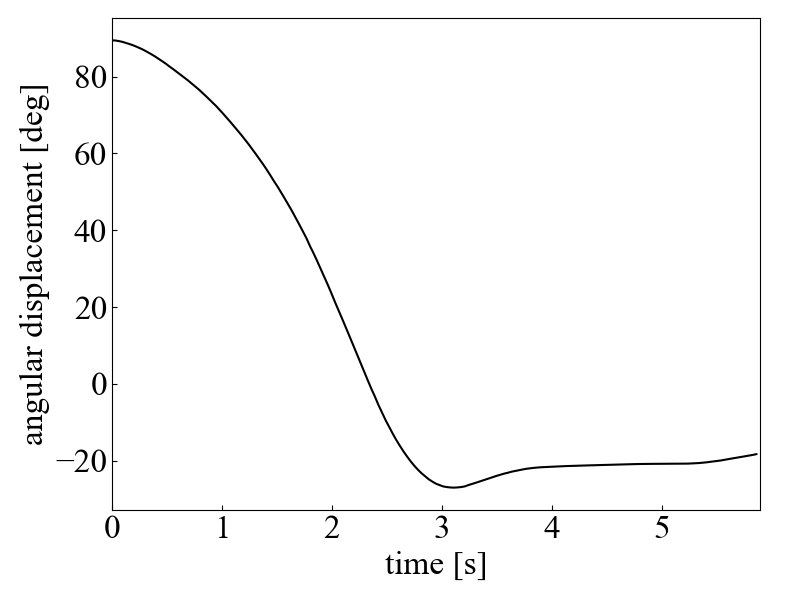
\includegraphics[width=\columnwidth]{./figure/PDdeg.png}
	  \caption{PD制御の角度推移}
	  \label{fig:PDdeg}
	\end{minipage}
	\hspace{5mm}
	\begin{minipage}{0.43\columnwidth}
	  \centering
	  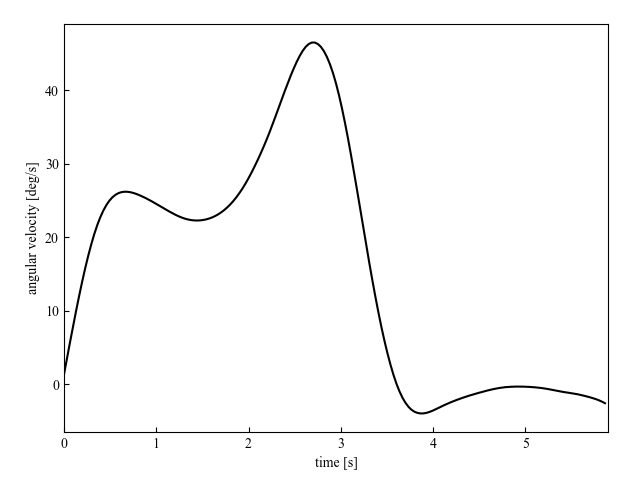
\includegraphics[width=\columnwidth]{./figure/PDdegpers.png}
	  \caption{PD制御の角速度推移}
	  \label{fig:PDdegpers}
	\end{minipage}
  \end{figure}

  \subsection{PID制御}
  \subsubsection{実験方法}
  \subsubsection{実験結果}

\begin{figure}[h]
	\centering
	\begin{minipage}{0.43\columnwidth}
	  \centering
	  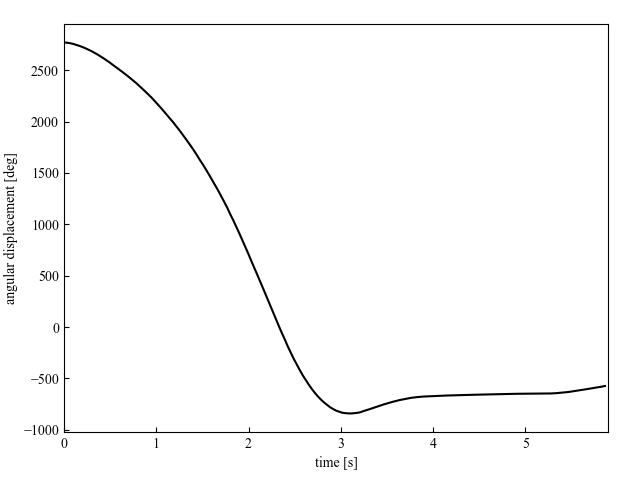
\includegraphics[width=\columnwidth]{./figure/PIDdeg.png}
	  \caption{PID制御の角度推移}
	  \label{fig:PIDdeg}
	\end{minipage}
	\hspace{5mm}
	\begin{minipage}{0.43\columnwidth}
	  \centering
	  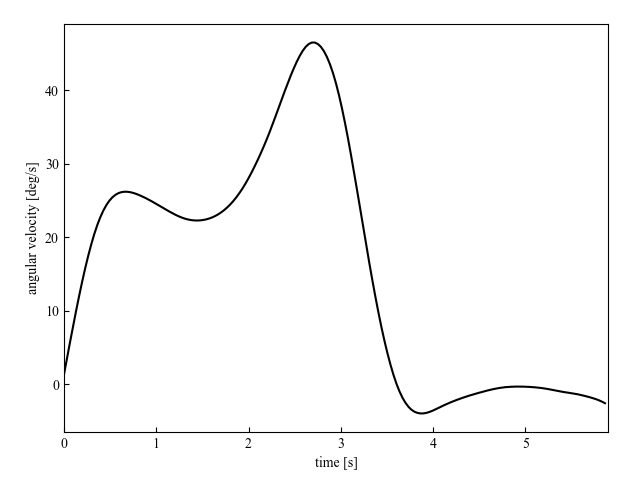
\includegraphics[width=\columnwidth]{./figure/PIDdegpers.png}
	  \caption{PID制御の角速度推移}
	  \label{fig:PIDdegpers}
	\end{minipage}
\end{figure}

\subsection{B-dot制御則}
\subsubsection{実験方法}
\subsubsection{実験結果}

\begin{figure}[h]
	\centering
	\begin{minipage}{0.43\columnwidth}
	  \centering
	  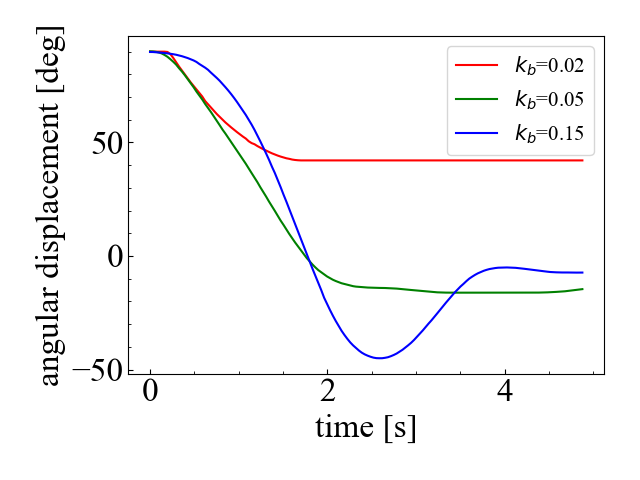
\includegraphics[width=\columnwidth]{./figure/kb5deg.png}
	  \caption{B-dot制御の角度推移}
	  \label{fig:kb5deg}
	\end{minipage}
	\hspace{5mm}
	\begin{minipage}{0.43\columnwidth}
	  \centering
	  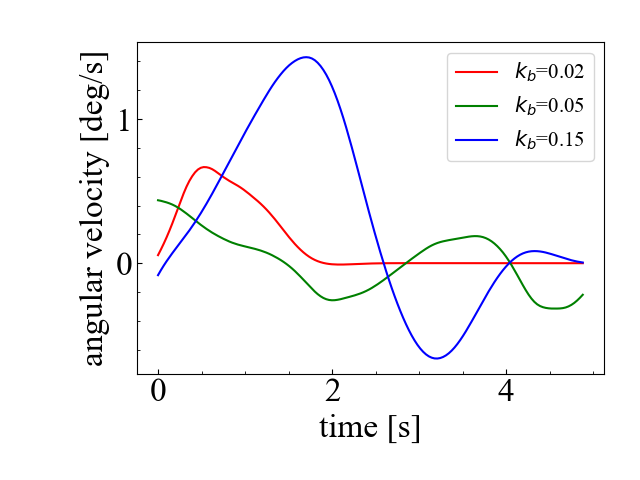
\includegraphics[width=\columnwidth]{./figure/kb5degpers.png}
	  \caption{B-dot制御の角速度推移}
	  \label{fig:kb5degpers}
	\end{minipage}
\end{figure}

\newpage

\subsection{クロスプロダクト則}
\subsubsection{実験方法}
\subsubsection{実験結果}

\begin{figure}[h]
	\centering
	\begin{minipage}{0.43\columnwidth}
	  \centering
	  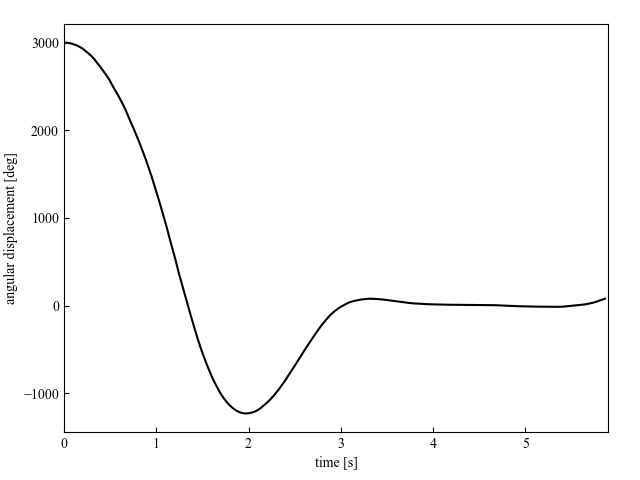
\includegraphics[width=\columnwidth]{./figure/crossdeg.png}
	  \caption{B-dot制御の角度推移}
	  \label{fig:crossdeg}
	\end{minipage}
	\hspace{5mm}
	\begin{minipage}{0.43\columnwidth}
	  \centering
	  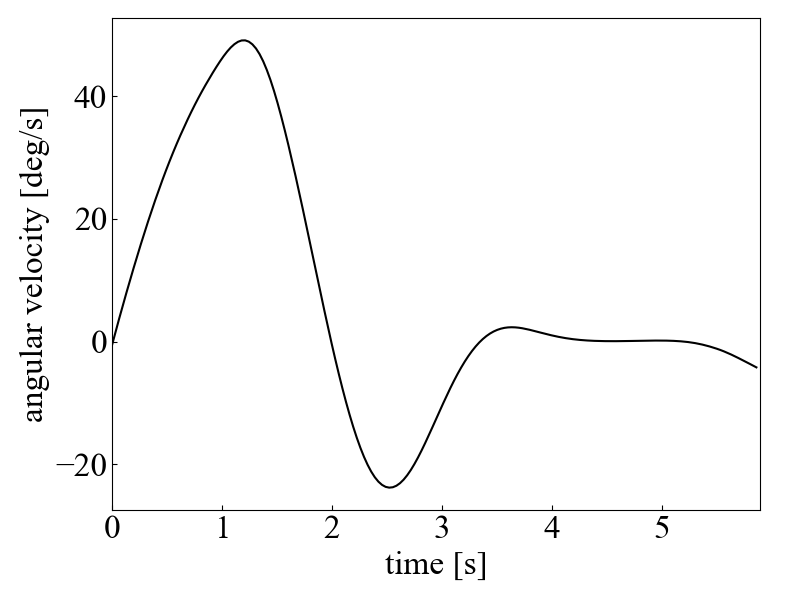
\includegraphics[width=\columnwidth]{./figure/crossdegpers.png}
	  \caption{B-dot制御の角速度推移}
	  \label{fig:crossdegpers}
	\end{minipage}
\end{figure}


\subsection{考察}

\newpage
\section{結論}
\subsection{本研究のまとめ}
\subsection{今後の展望}